\documentclass[a4paper, czech]{article}

\title{Úloha č.1: V-A charakteristiky polovodičových diod}
\author{Karolína Andrea Šebestová}
\date{Datum měření: 15.2.2024}

\usepackage[czech]{babel}
\usepackage{indentfirst}
\usepackage{graphicx}
\usepackage{float}
\usepackage[margin=1.5cm]{geometry}
\usepackage{booktabs}
\usepackage{amsmath}

\begin{document}
\maketitle
\section[short]{Teoretický úvod}
Polovodičová dioda je součástka založená na přechodu P-N nebo přechodu kov-polovodič (Schottkyho dioda). Její základní vlastností je vedení elektrického proudu pouze jedním směrem. Při zapojení v tomto tzv. propustném směru, je na anodě kladné napětí UF proti katodě a diodou protéká proud IF. Je-li dioda zapojena v tzv. závěrném směru, je přiložené napětí UR pólováno opačně, tj. na anodě záporné oproti katodě. V tomto stavu proud diodou prakticky neprotéká (pouze malý závěrný proud IR).
\begin{figure}[H]
  \centering
  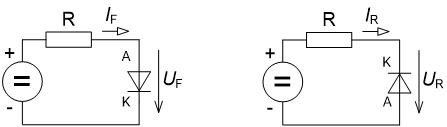
\includegraphics{zapojeni_diody}
  \caption{Zapojení diody v propustném a v závěrném směru}
  \label{obr:1}
\end{figure}

Základním popisem chování polovodičové diody je její voltampérová (V-A) charakteristika, tedy závislost proudu diodou na napětí na diodě, která má tvar dle Obr. 2.
\begin{figure}[H]
  \centering
  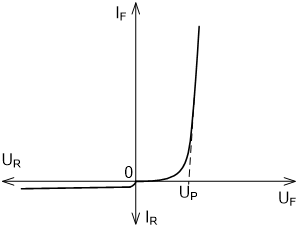
\includegraphics{va_charakteristika}
  \caption{Voltampérová charakteristika diody}
  \label{obr:2}
\end{figure}

\section[short]{Seznam přístrojů}
\begin{enumerate}
  \item 1x Zdroj Agilent E3620A
  \item 2x Multimetr Keysight 34461A
\end{enumerate}


\pagebreak

\section[short]{Úkoly měření}
\begin{enumerate}
  \item Sestavte zapojení podle Obr. \ref{obr:3} Jako voltmetr a ampérmetr použijte multimetry E34401A nebo E34461A. Vstupní svorky multimetrů pro měření napětí jsou horní dvě vpravo. Pro měření proudu na multimetrech stiskněte modré tlačítko Shift a poté tlačítko, nad kterým je modře DC I. Vstupní svorky multimetrů pro měření proudu jsou dolní dvě vpravo. Jako stejnosměrný zdroj použijte E3620A. Změnu z propustného do závěrného směru realizujte přehozením vývodů napájecího zdroje (znaménka u zdroje na Obr. \ref*{obr:3} v závorce). Změřte závislost proudu diodou na napětí, tedy voltampérovou charakteristiku, v propustném a závěrném směru. Proveďte měření pro všechny diody k dispozici, tj. křemíkovou 1N4148, Schottkyho BAT42 a LED. Černý proužek na diodě značí katodu, u LED je katoda označena plochou částí rozšíření na spodu pouzdra a kratším vývodem. Charakteristiku změřte v 10 až 15 bodech v každém směru. V oblasti zlomu charakteristiky měřte s menším krokem, ať můžete měřené body v grafu vhodně spojit hladkou čarou. V propustném směru ukončete měření při dosažení $I_{Fmax} = 10 mA$, v závěrném směru při $U_{Rmax} = 10 V$.
  \item Charakteristiky všech diod v propustném i závěrném směru zakreslete do společného grafu podobně jako na Obr. \ref*{obr:2} Jelikož jsou závěrné proudy diod mnohem menší než propustné, zvolte na ose závěrného proudu $I_R$ jemnější měřítko. Pokud grafy vykreslujete na počítači, kde nelze zvolit různá měřítka svislé osy, vykreslete propustnou a závěrnou část v samostatných grafech. Zakreslete do grafů prahová napětí jednotlivých diod $U_P$ a tato napětí odečtěte. Charakteristiky vzájemně porovnejte. 
\end{enumerate}
\begin{figure}[H]
  \centering
  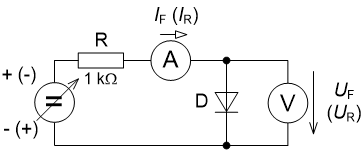
\includegraphics{zapojeni_mereni.png}
  \caption{Zapojení pro měření V-A charakteristiky diody}
  \label{obr:3}
\end{figure}
\section[short]{Naměřené hodnoty}
V této sekci se nachází šest tabulek. Každému typu diody náleží dvě tabulky, které popisují naměřenou V-A charakteristku v propustném, respektive v závěrném směru.

Slovní popis symbolů veličin:
$I_F$ - proud procházející diodou zapojenou v propustném směru;
$U_F$ - napětí na diodě zapojené v propustném směru;
$I_R$ - proud procházející diodou zapojenou v závěrném směru;
$U_R$ - napětí na diodě zapojené v závěrném směru

\subsection[short]{Křemíková dioda 1N4148}
\begin{table}[H]
  \resizebox{\textwidth}{!}{%
  \begin{tabular}{l||lllllllllllllll}
  \toprule
  $I_F\ (mA)$ & 0     & 0,25  & 0,5   & 0,75  & 0,9   & 1     & 2     & 3     & 4     & 5     & 6     & 7     & 8     & 9     & 10    \\
  \midrule
  $U_F\ (V)$  & 0 & 0,527 & 0,561 & 0,582 & 0,592 & 0,599 & 0,634 & 0,656 & 0,673 & 0,686 & 0,697 & 0,707 & 0,716 & 0,723 & 0,730 \\
  \bottomrule  
  \end{tabular}%
  }
  \caption{Naměřené hodnoty V-A charakteristiky diody 1N4148 v \underline{propustném} směru}
  \label{tab:1}
\end{table}

\begin{table}[H]
  \resizebox{\textwidth}{!}{%
  \begin{tabular}{l||lllllllllllllll}
  \toprule
  $U_R\ (V)$  & 0     & 0,1   & 0,25  & 0,5   & 1     & 2     & 3     & 4     & 5     & 6     & 7     & 8     & 9     & 10      \\
  \midrule
  $I_R\ (\mu A)$ & 0 & 0,011 & 0,027 & 0,053 & 0,106 & 0,205 & 0,303 & 0,403 & 0,505 & 0,603 & 0,703 & 0,804 & 0,903 & 1,004   \\
  \bottomrule  
  \end{tabular}%
  }
  \caption{Naměřené hodnoty V-A charakteristiky diody 1N4148 v \underline{závěrném} směru}
  \label{tab:2}
\end{table}

\subsection[short]{Schottkyho dioda BAT42}
\begin{table}[H]
  \resizebox{\textwidth}{!}{%
  \begin{tabular}{l||lllllllllllllll}
  \toprule
  $I_F\ (mA)$ & 0 & 0,1   & 0,25  & 0,5   & 0,75  & 1     & 2     & 3     & 4     & 5     & 6     & 7     & 8     & 9     & 10    \\
  \midrule
  $U_F\ (V)$ & 0 & 0,179 & 0,202 & 0,222 & 0,233 & 0,239 & 0,259 & 0,271 & 0,279 & 0,286 & 0,292 & 0,297 & 0,301 & 0,305 & 0,309 \\
  \bottomrule  
  \end{tabular}%
  }
  \caption{Naměřené hodnoty V-A charakteristiky diody BAT42 v \underline{propustném} směru}
  \label{tab:3}
\end{table}

\begin{table}[H]
  \resizebox{\textwidth}{!}{%
  \begin{tabular}{l||lllllllllllllll}
  \toprule
  $U_R\ (V)$ & 0 & 0,1   & 0,25  & 0,5   & 1     & 1,5   & 2     & 3     & 4     & 5     & 6     & 7     & 8     & 9     & 10    \\
  \midrule
  $I_R\ (\mu A)$ & 0 & 0,118 & 0,141 & 0,173 & 0,238 & 0,297 & 0,359 & 0,473 & 0,589 & 0,7   & 0,814 & 0,924 & 1,035 & 1,148 & 1,257   \\
  \bottomrule  
  \end{tabular}%
  }
  \caption{Naměřené hodnoty V-A charakteristiky diody BAT42 v \underline{závěrném} směru}
  \label{tab:4}
\end{table}

\subsection[short]{LED (červená)}
\begin{table}[H]
  \resizebox{\textwidth}{!}{%
  \begin{tabular}{l||lllllllllllllll}
  \toprule
  $I_F\ (mA)$ & 0 & 0,1   & 0,25  & 0,5   & 1     & 2     & 3     & 4     & 5     & 6     & 7     & 8     & 9     & 10    \\
  \midrule
  $U_F\ (V)$  & 0 & 1,625 & 1,66  & 1,686 & 1,709 & 1,737 & 1,754 & 1,768 & 1,777 & 1,786 & 1,794 & 1,802 & 1,808 & 1,814 \\
  \bottomrule  
  \end{tabular}%
  }
  \caption{Naměřené hodnoty V-A charakteristiky LED v \underline{propustném} směru}
  \label{tab:5}
\end{table}

\begin{table}[H]
  \resizebox{\textwidth}{!}{%
  \begin{tabular}{l||lllllllllllllll}
  \toprule
  $U_R\ (V)$  & 0 & 0,5   & 1     & 2     & 3     & 4     & 5     & 6     & 7     & 8     & 9     & 10  \\
  \midrule
  $I_R\ (\mu A)$ & 0 & 0,053 & 0,103 & 0,202 & 0,308 & 0,407 & 0,508 & 0,607 & 0,708 & 0,805 & 0,904 & 1,001   \\
  \bottomrule  
  \end{tabular}%
  }
  \caption{Naměřené hodnoty V-A charakteristiky LED v \underline{závěrném} směru}
  \label{tab:6}
\end{table}

\section[short]{Grafy}

Naměřené hodnoty byly vyneseny do společného grafu V-A charakteristiky, kde jsou křivky jednotlivých diod barevně rozlišeny (viz. legenda).
V prvním kvadrantu jsou vyneseny hodnoty veličin naměřené na diodě v propustném směru.
Naměřené hodnoty v závěrném směru jsou pak vyneseny do třetího kvadrantu.

Dva nejvyšší body každé závislosti byly použity na sestrojení přímky, která tvoří tečnu k lineární části křivky.
Je vyznačena růžovou barvou. Její průsečík s horizontální osou je hodnotou prahového napětí diody.

\begin{figure}[H]
  \centering
  \textbf{V-A charakteristika diod 1N4148, BAT42 a LED}\par\medskip
  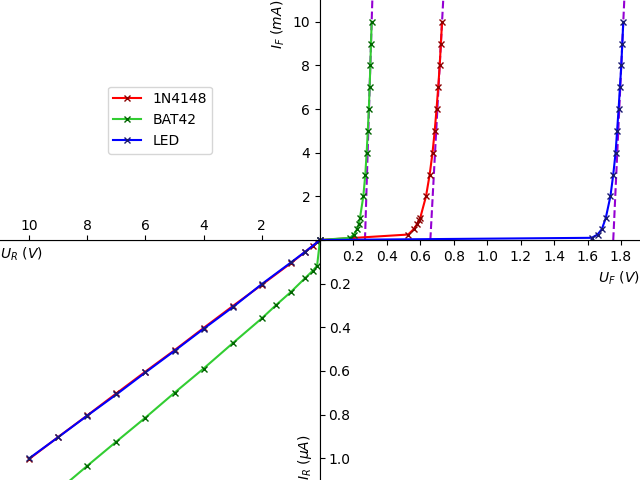
\includegraphics{va_charakteristika_final.png}
  \caption{Společná V-A charakteristika všech tří měřených diod}
  \label{obr:4}
\end{figure}

\begin{table}[H]
  \centering
  \begin{tabular}{lc}
  \toprule
  Typ diody  & $U_P\ (V)$ \\
  \midrule
  1N4148 & 0,66     \\
  BAT42  & 0,27     \\
  LED    & 1,75    \\
  \bottomrule
  \end{tabular}
  \caption{Hodnoty prahového napětí $U_P$ jednotlivých diod odečtené z grafu}
\end{table}

\section[short]{Závěr}

Porovnáním jednotlivých grafických charakteristik se ukazuje, že prahová napětí $U_P$ jednotlivých diod se od sebe významně liší.
Nejnižší prahové napětí z nich má Schottkyho dioda: $U_P = 0,27V$.
Úbytek napětí na Schottkyho diodě se na měřeném rozsahu pomalu blížil k hodnotě $0,3V$.
Prahové napětí křemíkové diody bylo o něco vyšší: $U_P = 0,66V$.
Úbytek napětí na křemíkové diodě se pak blížil k hodnotě $0,7V$.
Nejvyšší prahové napětí má LED: $U_P = 1,75$. Za zmínku stojí také fakt, že LED počas měření svítila již při relativně malých hodnotách proudu.
Ubytek napětí na LED se blížil k hodnotě $1,8V$

V závěrném směru je V-A charakteristika všech diod poměrně lineární.
"Ohyb" křivky je patrný pouze u Schottkyho diody.
U křemíkové diody a LED je charakteristika V-A charakteristika prakticky úplně lineární a to nejspíše proto, že na měřeném rozsahu není možné jasně odhalit velmi malý "ohyb" v křivce.
Pozoruhodné je i to, že V-A charakteristika křemíkové diody a LED v závěrném směru je téměř totožná.
V přiženém grafu se křivky i naměřené body překrývají.

\end{document}